\documentclass[a4paper,10pt,twocolumn,fleqn]{jsarticle}

\usepackage{sice_q_style}       %sice九州支部学術講演会用原稿スタイル
\usepackage{graphicx}
\usepackage{amsmath,amssymb,epsf}

\renewcommand{\floatpagefraction}{1}
\renewcommand{\topfraction}{1}
\renewcommand{\bottomfraction}{1}
\renewcommand{\textfraction}{0}

\def\vec#1{\mbox{\boldmath$#1$}}
\def\RealNumSet{\Bbb R}
\def\IntSet{\Bbb Z} 
\def\NatSet{\Bbb N}
\def\argmax#1{\underset{#1}{\mbox{argmax~}}}
\def\sgn#1{\mbox{sgn($#1$)}}
\def\sgn{\mbox{sgn}}
\def\argmin#1{\underset{#1}{\mbox{argmin}}}
\def\leqq{\le}
\def\geqq{\ge}
\def\deltah{\delta\vec{h}}
\def\norm#1{\Vert#1\Vert}
\def\reftable#1{Table~\ref{#1}}

\def\R{{\Bbb R}}
\def\ltheta{{\theta_{\mbox{\small lower}}}}
\def\utheta{{\theta_{\mbox{\small upper}}}}
\def\ltheta{{\theta_{\mbox{\small lower}}}}

\def\dth{{d_{\mbox{th}}}}
\def\Ith{{I_{\mbox{th}}}}
\def\cth{{c_{\mbox{th}}}}
\def\sth{{s_{\mbox{th}}}}
\def\Hth{{H_{\mbox{th}}}}
\def\RealNumSet{\Bbb R}
\def\myepsfile#1#2{\epsfile{file=#1, scale=#2}}
\def\myepsfile#1#2{\scalebox{#2}{\includegraphics{#1}}}
\def\vec#1{\mbox{\boldmath$#1$}}
\def\sgn#1{\mbox{sgn($#1$)}}
\def\c#1{^{#1}}
\def\argmin#1{\underset{#1}{\mbox{argmin~}}}
\def\expect#1{\langle #1 \rangle}
\def\expect#1{\overline{#1}}
\def\expect#1{E(#1)}
\def\expect#1#2{\langle{#1}\rangle_{#2}}
\def\expect#1#2{{E_{#2}(#1)}}
%%%%%%%%%%%

\newcommand{\abst}[1]{%
\date{\parbox{0.9\textwidth}{\normalsize\parindent=1em%
\vspace{0.5cm}
%\begin{center}{\bf 概要} \end{center}%
\vspace{-0.2cm}#1}}}
\pagestyle{empty}

\begin{document}

\twocolumn[%
\begin{center}
%%%%%%%%%%%%%%  題目(日本語)  %%%%%%%%%%%%%
%\hspace*{3zw}%zw:全角文字幅
%\begin{tabular*}{210mm}{@{}c@{}}
{\Large \textbf{反射波や回折波を含むGPS信号を用いる移動ロボットの状態推定のてすと}}

\vspace*{1zw}
\hspace*{100mm}九州工業大学 ○西田~健だよ
\vspace*{1zw}

%\hspace*{3zw}
%%%%%%%%%%%%%%  題目(英語)  %%%%%%%%%%%%%
 {\textbf{Mobile Robot's State Estimation using 
 Reflected and Diffracted Waves of a GPS Signal
 }}\\
%\vspace*{-2mm}
%\end{tabular*}
%\hspace*{3zw}
%%%%%%%%%%%%%%  著者(英語)  %%%%%%%%%%%%%
\vspace*{1zw}
 Takeshi NISHIDA\\ Kyushu Institute of Technology\\
\end{center}

%%%%%%%%%%%%%%%  abstract  %%%%%%%%%%%%%%
\begin{center}
\begin{tabular*}{160mm}{@{}p{160mm}@{}}
%\small 
{\bf Abstract} : 
 A method for improving a mobile robot's state
 estimation accuracy using the statistical character of
 the reflected and diffracted waves of a GPS (global positioning system)
 signal is proposed. 
%
% With the proposed method, the effective use of GPS signal containing
% the rejected noise by the conventional method is made possible, and the
% estimation accuracy of states of the robot in shadow area of GPS
% satellite can be improved. 
%
 Furthermore, 
 the control system of an autonomous mobile
 robot incorporating the proposed state estimation method is developed,
 and the performance of the proposed methods is verified via simulation.
\end{tabular*}
\end{center}
]

\section{はじめに}
\label{intro}
%
\vspace{-2mm}
Global Navigation Satellite System(GPS)は屋外移動ロボットの自己位置計
測に広く利用される.
%
%原理的には,ロボットに搭載されたGPSアンテナで信号を直接受信できるGPS衛星
%が4以上あれば自己位置計測が可能であり\cite{BH},より多くの可視衛星からの
%受信により測位品質が向上できる\cite{yamazaki}.
%
一般に,信号をアンテナで直接受信できるGPS衛星を可視衛星,それ以外を不可視衛星と呼び,
4以上の可視衛星が存在しない地上領域を衛星の陰と呼ぶ.
%
都市部などで周囲に高い建造物が存在する状況では,GPS信号に反射や回折が生
ずることで衛星の陰が数多く発生するため,計測誤差が飛躍的に大きくなる.
%
%\begin{figure}[bp]
% \centering
% 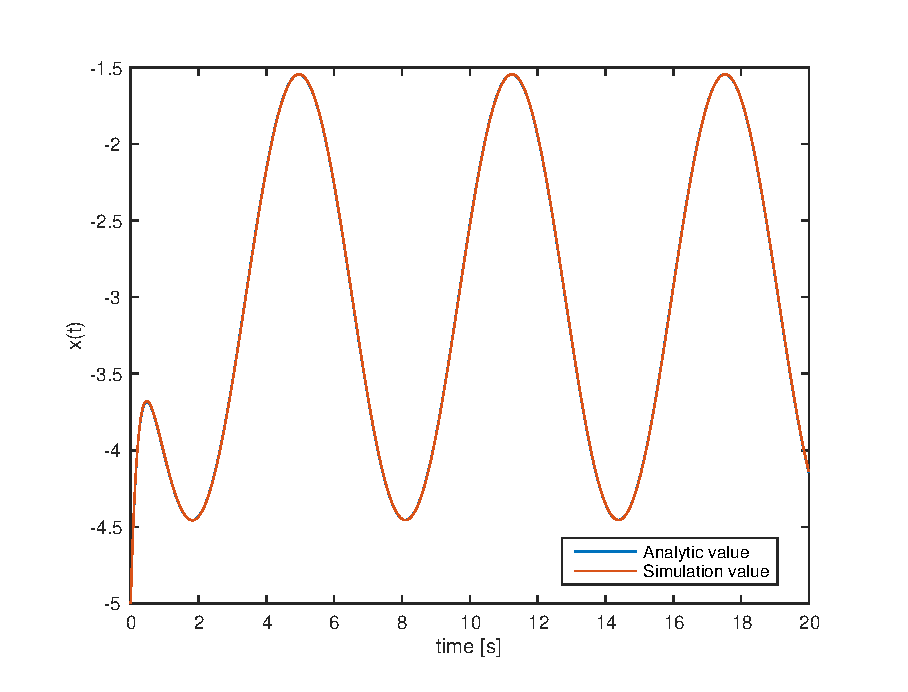
\includegraphics[width=60mm]{./fig/multi.eps}
% \caption{GNNS signal from an invisible satellite.}
% \label{fig:multi}
%\end{figure}
%
%この問題を解決する最も一般的な手法は,デッドレコニングや地図情報の参照に
%よる状態推定手法であり,車載ナビゲーションシステムとして広く用いられる
%\cite{p-robo}.
%
%この手法ではまず,GPS信号について可視GPS衛星からの直接波と不可視GPS衛星
%からの反射波や回折波などが分別される\cite{maier}.
%
%十分な数の可視衛星からの信号が得られない場合にはGPS信号の利用は停止され,
%オドメトリと地図情報の参照によるデッドレコニングが実行される.
%
%しかしデッドレコニングには,誤差の累積と,それをキャンセルする手段が無
%いという問題があるため,長時間の利用は困難である\cite{Bekey}.
%
%一方,3次元地図を利用するGPS計測の高精度化手法が提案されている
%\cite{yamazaki}.
%
%この手法では,高さ方向の情報を有する市街地地図を利用することで,GPS衛星
%の可視・不可視を判定する.
%
%さらに,衛星の陰でのロボットの動作をパーティクルフィルタ(PF: particle
%filter)\cite{kita,Doucet}によって推定する.
%
%しかし,この手法は3次元地図情報とGPS衛星の方位を正確に把握し,衛星
%の陰がどこに存在するかを算出する必要があるため,汎用性の面で課題が残され
%ている.
%
そこで
本論文では,GPS信号の反射波および回折波の統計的性質を用
いることで,移動ロボットの状態推定精度を向上する手法を提案する.
%
まず,反射波および回折波を含むGPS信号は,真の位置情報と時変ガウス分布に
従うノイズの和で表されると仮定する.
%%%
この仮定に基づき,GPS信号の時変バイアスをKF(Kalman filter)により推定
し,さらにそれを利用したサンプリングと尤度評価を実行するPF(particle
filter)を構成する.
%%%
この状態推定機構により,従来は棄却されていた反射波や回折波を含むGPS
信号の効果的な利用が可能になり,衛星の陰におけるロボットの状態量推定の精度
向上が可能になる.
%%
%さらに,提案する状態推定機構を組み込んだ自律走行ロボットの走行制御系を構
%成し,これが有効に動作することを示す.
%
%本手法は,地形の2次元もしくは3次元情報を必要としない手法であるた
%め,汎用性が高いことが特長である.

%本論文の構成は次の通りである.
%まず,\ref{sec:model}節において本論文で扱う移動ロボットの確率モデル
%を示し,\ref{sec:cntl}節において,PFを用いる状態推定手法とフィードバック
%制御手法を示す.
%
%さらに,\ref{sec:sim}節において数値シミュレーションにより提案手法の有効
%性をKFとの比較によって評価する.
%そして最後に\ref{sec:con}節において本論文の結論を述べる.
\vspace{-5mm}
\section{移動ロボットの確率モデル\label{sec:model}}
\vspace{-2mm}
\subsection{キネマティクスモデル}
\vspace{-2mm}
前輪操舵後輪駆動型の4輪移動ロボットを制御対象とする.
%
このロボットはディファレンシャル式の駆動輪を有し,回転運動における後輪の
滑りが発生しない.
%
ロボットの真の状態量を,原点を$O$とする慣性座標系$O-XY$における位置と角度
によって
$
 \vec{x}_k\triangleq
   [ \begin{matrix} x_k& y_k&\theta_k \end{matrix} ]^T 
   =[ \begin{matrix} \vec{z}^T_k& \theta_k \end{matrix} ]^T 
$
と定義する.
ここで,$k=0,1,2,\cdots$は離散時刻,
$\vec{z}_k\triangleq[\begin{matrix}x_k& y_k \end{matrix}]^T$はロボットの
後輪車軸中央に設定されたロボットの中心の位置,$\theta_k$はロボットの進行方向と
$X$軸との角度,$l$は前後車輪軸間の距離を表す.
%
次に,動作指令入力を
$
 \vec{u}_k \triangleq
 [ \begin{matrix} v_k& \phi_k \end{matrix} ]^T
$
とする.ここで$v_k$は駆動輪の回転によって発生する進行方向速度であ
り,$\phi_k$は反時計回りを正とする前輪の操舵角を表す.
%これらのロボットのパラメータと座標系の関係をFig.\ref{fig:model}に示す.
%
%\begin{figure}[bp]
% \centering
% \includegraphics[width=40mm]{./fig/axis.eps}
% \caption{State of a mobile robot in the world coordinate system.}
% \label{fig:model}
%\end{figure}
%%
このロボットの離散時間状態方程式は以下で表せる\cite{p-robo}.
\begin{align}
 \vec{x}_{k+1}
 &=\vec{f}(\vec{x}_{k},\vec{u}_{k})\nonumber\\
 &\hspace{-5mm}=\vec{x}_{k}+\left[
  \begin{matrix}
   \frac{v_k}{\omega_k}\left\{\sin(\theta_{k}+\omega_k\Delta)
   -\sin\theta_{k}\right\}\\
   -\frac{v_k}{\omega_k}\left\{\cos(\theta_{k}+\omega_k\Delta)
   -\cos\theta_{k}\right\}\\
   \omega_k\Delta
  \end{matrix}
  \right] 
 \label{eq:state}
\end{align}
ここで,$ \omega_k\triangleq (v_k/l)\tan\phi_k$
であり,$\Delta$はサンプリング周期である.
\vspace{-5mm}
\subsection{確率的離散状態空間モデル}
\vspace{-2mm}
現実的なロボットでは,駆動系のバックラッシュや劣化,さらに路面の傾きや滑
りなどの影響により,制御入力にノイズが加わる場合がある.
%
したがって,平均値が0のガウス分布に従う外乱が動作司令入
力に混入するとして以下のようにモデル化する\cite{p-robo}.
\begin{align}
 \hat{v}_k&\triangleq v_k+\varepsilon_v, \ \ 
 \varepsilon_v \sim 
 \mathcal{N} (0,\alpha_{1} v^2_k+\alpha_2 \phi^2_k) \\
 \hat{\phi}_k&\triangleq \phi_k+\varepsilon_{\phi}, \ \ \varepsilon_\phi \sim
 \mathcal{N}(0,\alpha_3 v^2_k+\alpha_4\phi^2_k) 
\end{align}
ここで,$\alpha_i~(i=1,2,3,4)$はノイズの性質を決定する正の定数である.
%
また同様に,路面凹凸などによってロボットの方位角に外乱が加わることを考慮
し,以下のように方位角の推移をモデル化する.
\begin{align*}
 \hat{\theta}_{k+1}
 &=\hat{\theta}_{k}+(\hat{\omega}_k +\varepsilon_\gamma)\Delta, \ \
 \varepsilon_\gamma\sim 
 \mathcal{N}(0,\alpha_5 v^2_k+\alpha_6 \phi^2_k )
\end{align*}
ここで,
$\hat{\omega}_k\triangleq (\hat{v}_k/l)\tan\hat{\phi}_k$,
$\alpha_j~(j=5,6)$はノイズの性質を決定する正の定数
である.また,記述の簡単のために$\vec{\varepsilon}_k\triangleq
[
\begin{matrix}
 \varepsilon_v& \varepsilon_\phi& \varepsilon_\gamma 
\end{matrix}
]^T$と記述する.

以上の関係を用いると,式(\ref{eq:state})は確率遷移モデル
として次のように記述できる.
\begin{align}
 \hat{\vec{x}}_{k+1}
&=p_f\left(\hat{\vec{x}}_{k+1} \big\vert
 \hat{\vec{x}}_k, \vec{u}_k \right)\nonumber\\
&\hspace{-5mm}= \hat{\vec{x}}_{k}+\left[
  \begin{matrix}
   \frac{\hat{v}_k}{\hat{\omega}_k}
   \left\{\sin(\hat{\theta}_{k}
   +\hat{\omega}_k\Delta)
   -\sin\hat{\theta}_{k}\right\}\\
   -\frac{\hat{v}_k}{\hat{\omega}_k}
   \left\{\cos(\hat{\theta}_{k}
   +\hat{\omega}_k\Delta)
   -\cos\hat{\theta}_{k}\right\}\\
   (\hat{\omega}_k+\varepsilon_\gamma)\Delta
  \end{matrix}
 \right]
 \label{eqn:prob}
\end{align}
ここで,$\hat{\vec{x}}_{k}\triangleq [\hat{x}_k\ \ \hat{y}_k\ \
\hat{\theta}_k]^T$は確率的に推移する要素を含む状態量を表す.
\vspace{-2mm}
\subsection{観測モデル}
\vspace{-2mm}
移動ロボットは,搭載したGPSアンテナによって各離散時刻における自己
位置
$\vec{z}^{\text{GPS}}_{k}\triangleq
[\begin{matrix}
  x^{\text{GPS}}_k &
  y^{\text{GPS}}_k 
 \end{matrix}]^T$
を
$
 \vec{z}^{\text{GPS}}_k = \vec{z}_k +  \vec{\xi}_k
 \label{eqn:zgps}
$
として観測する.ここで
\begin{align}
 \vec{\xi}_k\sim 
 \begin{cases}
 \mathcal{N}(r_k,\vec{\Sigma}_s)  & \text{if in a shadow area} \\
 \mathcal{N}(0,  \vec{\Sigma}_b)  & \text{otherwise} 
 \end{cases}
 \label{eqn:www}
\end{align}
であり,周囲の環境によってバイアスと分散が変化するガウス分布に従うノ
イズである.
%
すなわち,衛星の陰ではバイアス$r_k$および分散
$\vec{\Sigma}_s=\text{diag}[\sigma_s^2, \sigma_s^2]$のガウス分布に従い,GPS信
号が直接観測できる領域ではバイアス0および分散
$\vec{\Sigma}_b=\text{diag}[\sigma_b^2, \sigma_b^2]$のガウス分布に従う.
一般に,衛星の陰ではGPS信号の分散が大きくなることから
$
\text{det}(\vec{\Sigma}_b)<\text{det}(\vec{\Sigma}_s)
$である.

次に,方位角の計測はGPS信号に含まれないため,ロボットの方位角は
以下のように算出し,これを観測値とする.
\begin{align}
\theta^{\text{GPS}}_k
 &=\tan^{-1}\left(
\frac{y^{\text{GPS}}_{k}-\hat{y}_{k-1}}{x^{\text{GPS}}_{k}-\hat{x}_{k-1}}
 \right)+\omega_{k-1}\Delta
\end{align}
これらの観測値をまとめて観測ベクトルとする.
\begin{align}
 \vec{h}(\hat{\vec{x}}_k)=
 \vec{y}_k^{\text{GPS}}\triangleq
 \left[
 \begin{matrix}
  x_k^{\text{GPS}} &y_k^{\text{GPS}} &\theta_k^{\text{GPS}} 
 \end{matrix}
 \right]^T
\end{align}
\vspace{-10mm}
\section{状態量推定と制御\label{sec:cntl}}
\vspace{-2mm}
\subsection{PFによる状態推定と制御}
\vspace{-2mm}
本研究で構成するロボット走行制御系の状態変数線図を
Fig.\ref{fig:system2}に示す.
\begin{figure}[bp]
 \centering
 \includegraphics[width=.8\linewidth]{fig/syssys.ps}
 \caption{State variable diagram of the regulator with a PF observer.}
 \label{fig:system2}
\end{figure}
%
これは,ロボットの速度一定のもとで操舵角のみを制御することにより,指
定された領域を順に通過することを目的として構成された制御系である.
%
この制御系では,ロボットの状態推移は非線形モデルで表され,GPS信号には時
変ガウス分布に従うノイズが混入する.
なお,GPS信号に混入する観測雑音の時間変化に関する事前知識は与えられない
とする.

%ここでGPS信号を用いた
%PFによる状態推定を行う多くの従来研究では,運動モデルに基づくサンプリング
%とGPS信号に基づく尤度評価が行われる.
%%
%このような尤度評価を用いた場合,運動モデルに基づくサンプリングとGPS信号の観測に突発的
%に大きな差異が発生する状況では,その時点で粒子が数多く存在する領域,すな
%わち運動モデルに従うサンプリングが行われる領域における推定が実行され,
%観測の変動は無視される.
%%
%この状況は,GPS信号のバイアスが短時間で0に戻る場合には有効に作用する.
%%
%しかし,時間の経過に伴って運動モデルには誤差が累積し,その後リサンプリン
%グが実行されると,GPS信号の観測領域に粒子が突発的に移動するため状態推定
%が不連続に変動し,それを用いるフィードバック制御系は不安定化する恐れがあ
%る.
%%
%したがって,
GPS信号のバイアスと分散が大きく変化する場合にも制御系を安定に
駆動し続けるためには,衛星の陰におけるGPS信号の統計的性質を状態推定器
に事前知識として組み込む必要がある.
%
そこでまず,KFを利用して出力信号からGPS信号のバイアスを推定する.
%
次に,衛星の陰におけるGPS信号の統計的性質を組み込んだPFにより,KFの推定
バイアスを利用した状態推定を行う.
%
さらに,そのPFの事後推定に基づいた制御入力を算出し,ロボットを制御する.
\vspace{-4mm}
\subsection{KFによるGPS信号のバイアス推定}
\vspace{-2mm}
式(\ref{eqn:www})によりモデル化される出力信号は,次のようなガウス分布に従
うノイズが混入する系として表される.
\begin{align}
 \vec{\eta}_{k+1}=\vec{A}\vec{\eta}_{k},\ \
 \vec{z}^{\text{GPS}}_{k}=\vec{C}\vec{\eta}_{k}+\vec{w}_k
\end{align}
ここで
\begin{align*}
 \vec{\eta}_k &\triangleq 
 \left[
 \begin{matrix}
  \hat{x}_k \\ \hat{v}_{xk} \\
  \hat{y}_k \\ \hat{v}_{yk}
 \end{matrix}
 \right],\ 
%
 \vec{A} \triangleq 
 \left[
 \begin{matrix}
  1 & \Delta & 0 & 0\\
  0 & 1 & 0 & 0\\
  0 & 0 & 1 & \Delta\\
  0 & 0 & 0 & 1 
 \end{matrix}
 \right],\ \ 
 \vec{C} \triangleq 
 \left[
 \begin{matrix}
  1 & 0 \\ 0 & 0 \\  0 & 1\\  0 & 0
 \end{matrix}
 \right]\\
 \vec{w}_k  &\sim \mathcal{N}(\vec{0},\vec{R}),\ \
%
\vec{R} \triangleq  
 \text{diag}\left[
 \begin{matrix}
  \sigma^2_c & \sigma^2_c 
 \end{matrix}
 \right]
\end{align*}
であり,$\hat{v}_{xk}$と$\hat{v}_{yk}$はそれぞれ$X$
軸および$Y$軸方向の速度,$\sigma^2_c$は$\vec{w}_k$のX軸方向とY軸方向の分
散である.
この系に対し,ガウス分布に従うノイズを除く目的でKFを適用し
$\vec{\eta}_k$を推定する.
%\begin{align}
% \vec{\eta}_k^- &=
% \vec{A}\vec{\eta}_{k-1}\\
% \vec{P}_k^- &=\vec{A}\vec{P}_{k-1}\vec{A}^T\\
% \vec{K}_k^-
% &=\vec{P}_k^-\vec{C}^T\left(\vec{C}\vec{P}_k^-\vec{C}^T+\vec{R}\right)^{-1}\\
% \vec{\eta}_k
% &=\vec{\eta}_k^-+\vec{K}_k\left(\vec{z}_k^{\text{GPS}}-\vec{C}^T\vec{\eta}_k^-\right)\\
% \vec{P}_k
% &=\left(\vec{I}-\vec{K}_k\vec{C}\right)\vec{P}_k^-
%\end{align}
ここで,より大きな分散に対応するために,前述の仮定より
$\sigma_c^2=\sigma_s^2$とおく.
%
さらに推定を利用して,GPS
信号のバイアスを
$
\hat{r}_k=\sqrt{\hat{x}_k^2+\hat{y}_k^ 2}
$
と推定する.
\vspace{-4mm}
\subsection{サンプリング}
\vspace{-2mm}
PFは$M$個の重み付けされた粒子集合
$\left\{\vec{x}^{(i)}_k,\pi_{k}^{(i)}\right\}^{M}_{i=1}$
により状態推定を行う.
ここで,$\vec{x}_{k}^{(i)}$は仮説を表す粒子の状態空間中の位置,
$\pi_{k}^{(i)}\geq 0$は粒子の重みである.
%
PFによる推定の手続きは,サンプリング,粒子の尤度評価,リサンプリングの3
ステップから成る.
ここでは,サンプリングについて詳細に述べる.

本研究では,粒子の移動と分布のための提案分布を次のように設計する.
\begin{align*}
 \tilde{\vec{x}}^{(i)}_k &\sim
p_q\left(\tilde{\vec{x}}^{(i)}_{k} \vert \vec{x}^{(i)}_{k-1}\right)
=
 \begin{cases}
  p_f\left(\tilde{\vec{x}}^{(i)}_{k} \vert \vec{x}^{(i)}_{k-1}\right) 
  & (95 \%)\\
  p_r\left(\tilde{\vec{x}}^{(i)}_{k} \vert \vec{x}^{(i)}_{k-1}\right)
  & (5 \% )
 \end{cases}
\end{align*}
このサンプリングにおいて,$p_f(\cdot)$は全体の95\%の粒子は前時刻$k-1$
の粒子分布と入力,システムノイズを考慮した式(\ref{eqn:prob})に基づくサン
プリングを行う.
%
%これは通常のPFのサンプリング方法であり,同様の手法が数多く提案されている.
%
一方,全体からランダムに選択された5\%の粒子は,以下に示すような
$p_r(\cdot)$に従うサンプリングを行う.
\begin{align}
 p_r\left(\vec{x}^{(i)}_{k} \vert \vec{x}^{(i)}_{k-1}\right)
 = \vec{f}\left(\vec{x}^{\text{est}}_{k-1},
  \vec{u}_{k-1}\right)+\vec{R}_\psi\vec{\rho}(\hat{r}_k)
\end{align}
ここで,$\vec{x}^{\text{est}}_{k-1}$は前時刻の事後推定,
\begin{align}
 \vec{\rho}(\hat{r}_k)&\triangleq [\rho(\hat{r}_k)\ \  0]^T,\ \ \ \rho(\hat{r}_k) \sim
 \mathcal{N}\left(\hat{r}_s,\sigma^2_b\right)\\
 \vec{R}_\psi&\triangleq  
 \left[
 \begin{matrix}
  \cos \psi & -\sin \psi \\
  \sin \psi & \cos \psi 
 \end{matrix}
 \right],\ \ \psi\in \text{rand}[0, 2\pi] 
\end{align}
であり,$p_q(\cdot)$でサンプリングされた粒子の重みは次のように与える.
\begin{align}
 \pi^{(i)}_k=\frac{1}{
 M\sqrt{2\pi\sigma_s^2}} \exp
 \left\{-\frac{1}{2}\frac{\rho(\hat{r}_k)^2}{\sigma_s^2}\right\}
\end{align}
すなわち,式(\ref{eq:state})のロボットの運動モデルに基づいて推定された状
態を基準として,$\mathcal{N}\left(\hat{r}_k,\sigma^2_b\right)$に従ってサ
ンプリングされた粒子を半径$\hat{r}_k$の同心円状にランダムに回転座標変換す
る.
%
これは,衛星の陰におけるロボットの状態推定の精度を向上させるためのサンプ
リングの工夫である.
%
%すなわち,式(\ref{eqn:zgps})と式(\ref{eqn:www})から分かるように,GPS衛星
%の陰にロボットが位置する場合にも,GPS信号は真の状態と観測ノイズの合成で
%表される.
%%
%したがって,観測ノイズに関する先見知識を利用することで衛星の陰
%におけるGPS信号も状態推定に利用可能になる.
%%
%本研究では,反射波や回折波を含むGPS信号は真の状態量と時変ガウス分布に従
%うノイズの和で表されるという仮定を$p_r(\cdot)$として表現し,PFの手順に
%組み込む.
%
これらのサンプリング手法の概要をFig.\ref{fig:movemove}に示す.
% 
\begin{figure}[bp]
 \centering
 \includegraphics[width=.7\linewidth]{./fig/move.eps}
 \caption{Schematic view of the sampling.}
 \label{fig:movemove}
\end{figure}

%従来手法では,ロボットがGPS衛星の陰に入りGPS信号のバイアスが移動してノイズ
%の分散が拡大する状況では,キネマティクスモデルのみに従う自己位置推定に切
%り替える手法が用いられる.
%しかし,この状況が長い時間継続する場合には,真の状態と推定の累積誤差によ
%り制御系が不安定化するという問題が発生する.
\vspace{-10mm}
\subsection{尤度評価}
\vspace{-2mm}
GPS衛星の直接波が観測できる領域でのGPS信号に基づく尤度関数
を以下のように与える.
\begin{align*}
 p_{\text{direct}}\left( \vec{y}^{\text{GPS}}_k
 \big\vert\vec{x}^{(i)}_k \right)&\nonumber\\
 & \hspace{-20mm}=
 \frac{2}{3}\cdot\frac{1}{2\pi\sigma_b^2}\left\{
 \exp\left(
 -\frac{d^2_x}{2\sigma_b^2}\right)
 +\exp\left(
 -\frac{d^2_y}{2\sigma_b^2}\right)\right\}\nonumber\\
 & \hspace{-15mm} +
 \frac{1}{3}\cdot\frac{1}{2\pi\sigma_p^2}\exp\left(
 -\frac{d_\theta^2}{2\sigma_p^2}\right)
\end{align*}
ここで,
$d_x=\delta\left( x_k^{(i)}-x^{\text{GPS}}_k\right)$,
$d_y=\delta\left( y_k^{(i)}-y^{\text{GPS}}_k\right)$,
$d_\theta =\delta\left(\theta_k^{(i)}-\theta^{\text{GPS}}_k \right)$
であり,$\delta(\cdot)$はディラクのデルタ関数である.
さらに,GPS衛星の陰領域でのGPS信号に基づく尤度関数
を以下のように与える.
\begin{align*}
  p_{\text{shadow}}
 \left(\vec{y}^{\text{GPS}}_k\big \vert\vec{x}^{(i)}_k \right)&\nonumber\\
 & \hspace{-30mm}=
 \frac{2}{3}\cdot\frac{1}{2\pi\sigma_s^2}\exp\left(
 -\frac{d_{xy}^2}{2\sigma_s^2}\right)
 +
 \frac{1}{3}\cdot\frac{1}{2\pi\sigma_p^2}\exp\left(
 -\frac{d_\theta^2}{2\sigma_p^2}\right)
\end{align*}
ここで,$
 d_{xy}=\vert \delta(z_k^{(i)}-z^{\text{GPS}}_k) \vert -\hat{r}_k$
である.
これらのモデルの合成により,GPS信号の観測モデルを以下のように構築する.
\begin{align*}
 p_h\left(
 \vec{y}^{\text{GPS}}_k \big \vert \vec{x}^{(i)}_k \right)&\nonumber\\
&\hspace{-20mm}=
 \frac{1}{2}
 p_{\text{direct}}\left( \vec{y}^{\text{GPS}}_k \big \vert \vec{x}^{(i)}_k\right)+
\frac{1}{2}
 p_{\text{shadow}}\left( \vec{y}^{\text{GPS}}_k \big \vert\vec{x}^{(i)}_k\right)
\end{align*}
%この尤度関数の概略をFig.\ref{fig:multi}に示す.
%\begin{figure}[bp]
% \centering
% \includegraphics[width=.8\linewidth]{./fig/like1.eps}
% \caption{Likelihood function of a measurement model.}
% \label{fig:multi}
%\end{figure}
また,この尤度関数を利用して粒子
$\tilde{\vec{x}}_{k}^{(i)}$の重み$\tilde{\pi}^{(i)}_{k}$を次の
ように更新する.
 \begin{align}
 \tilde{\pi}^{(i)}_{k} \propto
   \pi^{(i)}_{k-1}   p_h
 \left(\vec{y}^{\text{GPS}}_k \big \vert\vec{x}^{(i)}_k \right), \ \
  \left(\forall i \right)
\end{align}
ただし,この更新の後に$\sum_{i=1}^{M}\tilde{\pi}^{(i)}_{k}=1$となるよう
にすべての重みを正規化する.

以上の尤度評価の後にPFの事後推定が以下のように算出できる.
\begin{align}
 \vec{x}_k^{\text{est}}=\sum_{i=1}^M \pi^{(i)}_{k}\delta (\vec{x}^{(i)})
\end{align}
さらに,この事後推定を用いて制御入力が
$
 \phi_{k+1}=k_{\phi} 
 \left(\phi_k^* \ominus \phi_k\right)$
と導出される\cite{peter}.
ここで,
$
 v_k=\text{const.}
$
および
$
 \phi_k^*=\tan^{-1} \left\{
 \left(
 y^{\text{target}}_i-y^{\text{est}}_k
 \right)/
 \left(
 x^{\text{target}}_i-x^{\text{est}}_k
 \right)\right\}
$
,$\phi^*,\phi \in [0, 2\pi)$であり,$\ominus$は$[0, 2\pi)$における
小さい方の角度差,$k_\phi$はフィードバックゲインである.

\vspace{-4mm}
\subsection{リサンプリング}
\vspace{-2mm}
有効サンプルサイズ(ESS: effective sample size)\cite{Liu}に基づきリサンプリングの
実行を判断する.
\begin{align}
 ESS=\frac{1}{\sum_{i=1}^M\left(\tilde{\pi}_k^{(i)}\right)^2}
\end{align}
この値は,全粒子の重みが均等である場合に$ESS=M$となり,重み
の偏りが最も大きい場合に$ESS=1$となる.
適当なしきい値
$ESS_{\text{th}}$を設け,$ESS$の値がそれを下回ればリサンプリングを実行す
る.すなわち,
$\tilde{\pi}^{(i)}_{k}$の確率で$\vec{x}^{(i)}_{k}$を
復元抽出する.
  \begin{align}
   \vec{x}_k^{(i)} \sim
   \begin{cases}
    \tilde{\vec{x}}_k^{(1)} & \mathrm{with\ prob.} \ \ \tilde{\pi}_k^{(1)}\\
    \vdots & \vdots \\
    \tilde{\vec{x}}_k^{(M)} & \mathrm{with\ prob.} \ \ \tilde{\pi}_k^{(M)}
   \end{cases},
   \ \ (\forall i)
  \end{align}
その後,重みを
$
      \pi_k^{(i)}:= 1/M, \ (\forall i)
$
として均等化する.
ここで
``$:=$''は代入を意味する.
リサンプリングを行わない場合には,
$      \vec{x}_k^{(i)}:=\tilde{\vec{x}}_k^{(i)},\ \ 
      \pi_k^{(i)}:=\tilde{\pi}_k^{(i)}
$     とする.以上の処理によって新しい時刻の粒子の集合
$
  \left\{ \left( \vec{x}^{(m)}_k, \pi^{(m)}_{k} \right)
  \right\}_{m=1}^{M} 
$
が獲得される.この後に$k:=k+1$としてサンプリング手順に戻る.



\vspace{-4mm}
%%%%%%%%%%%%%%%%%%%%%%%%%%%%%%%%%%%%%%%%
\section{シミュレーション\label{sec:sim}}
%%%%%%%%%%%%%%%%%%%%%%%%%%%%%%%%%%%%%%%%
\vspace{-2mm}
%
ロボットはフィールド上に設定された8つのターゲッ
トを順番に通過するよう制御される.
%
ただし,ターゲットから0.5[m]以内にロボットが近接したと推定されたら,
目標ターゲットを次の順番のターゲットに移す.
%
%\begin{figure}[btp]
% \begin{center}
%  \includegraphics[width=.9\linewidth]{fig/conditions.ps}
% \end{center}
% \caption{Conditions of the simulation.}
% \label{fig:cond}
%\end{figure}
%
走行速度は$v_k=10$[m/s]で一定とした.
さらに,ロボット固有の各パラメータは次のように定めた:車体の長さ$l=1$[m],移動に
おける速度成分の雑音パラメータ$\alpha_1=\alpha_3=\alpha_5=3.0$,操舵角成
分の雑音パラメータ$\alpha_2=\alpha_4=\alpha_6=0.3$,フィードバッ
クゲイン$k_\phi=0.8$,サンプリングおよび制
御周期$\Delta=0.01$[s].

次に,GPS信号の雑音に関する各パラメータは次のように定めた:
$\sigma_b^2=0.0025$,$\sigma_s^2=0.1$,$\sigma_p^2=0.01$.
さらに,フィールドの$X<0$の領域がGPS信号の影領域であるとし,GPS
信号に加わるノイズのバイアスを$r_k=4$ [m] (const.)とした.
PFの粒子数は$M=1000$,ESSのしきい値は$ESS_{\text{th}}=5.0$とした.

提案手法による走行制御の結果の一部をFig.\ref{fig:res}に示す.
\begin{figure}[bp]
 \begin{center}
 \begin{tabular}{cc}
%  \includegraphics[width=.4\linewidth]{fig/p100.ps}&
  \includegraphics[width=.45\linewidth]{fig/r070.ps}& 
  \includegraphics[width=.45\linewidth]{fig/r190.ps}\\
  (a) time=200[s]& (b) time=300[s] \\
  \includegraphics[width=.45\linewidth]{fig/r260.ps}&
  \includegraphics[width=.45\linewidth]{fig/r300.ps}\\
  (c) time=400[s] &(d) time=500[s]
%  \includegraphics[width=.4\linewidth]{fig/p650.ps}\\
% (f) time=570[s]& (g) time=650[s]
\end{tabular}
 \end{center}
 \caption{State variable diagram of the regulator with RBPF.}
 \label{fig:res}
\end{figure}
これらの図より,提案手法では衛星の陰において,キネマティクスモデルに基づ
く粒子分布とバイアス推定に基づく同心円状の粒子分布が同時に存在することが
わかる.
このような粒子分布によって,反射や回折によって生ずるGPS信号の誤差を考慮
することが可能になっている.

次に,次のような一般的なPFの構成によるシミュレーションを比較のために行っ
た.
すなわわち,サンプリングはシキネマティクスモデルのみに従う.
\begin{align}
 \tilde{\vec{x}}^{(i)}_k &\sim
p_q\left(\tilde{\vec{x}}^{(i)}_{k} \vert \vec{x}^{(i)}_{k-1}\right)
=  p_f\left(\tilde{\vec{x}}^{(i)}_{k} \vert \vec{x}^{(i)}_{k-1}\right) 
\end{align}
さらに,GPS信号が直接観測できる場合の尤度関数のみを利用する.
\begin{align}
 p_h\left(
 \vec{y}^{\text{GPS}}_k \big \vert \vec{x}^{(i)}_k \right)=
 p_{\text{direct}}\left( \vec{y}^{\text{GPS}}_k \big \vert \vec{x}^{(i)}_k\right)
\end{align}
%これらの構成で駆動させた場合のロボットの走行制御の結果の一部を
%Fig.\ref{fig:res2}に示す.
%\begin{figure}[btp]
% \begin{center}
% \begin{tabular}{cc}
%  \includegraphics[width=.4\linewidth]{fig/q100.ps}&
%  \includegraphics[width=.4\linewidth]{fig/q198.ps}\\
%  (a) time=100[s]& (b) time=200[s] \\
%  \includegraphics[width=.4\linewidth]{fig/q330.ps}&
%  \includegraphics[width=.4\linewidth]{fig/q440.ps}\\
%  (c) time=330[s] & (d) time=440[s] \\
%  \includegraphics[width=.4\linewidth]{fig/q570.ps}&
%  \includegraphics[width=.4\linewidth]{fig/q650.ps}\\
%  (e) time=570[s] & (f) time=650[s]
%\end{tabular}
% \end{center}
% \caption{State variable diagram of the regulator with RBPF.}
% \label{fig:res2}
%\end{figure}
%
%一方で,従来手法では粒子分布の領域が狭く,影領域においてもGPS信号の周囲
%にはひとつも粒子が配置されていない様子がわかる.
提案手法と従来手法によるロボットの走行軌跡を,それぞれ
Fig.\ref{fig:track2}(a)と(b)に示す.
%\begin{figure}[bp]
%\begin{tabular}{cc}
% \includegraphics[width=.45\linewidth]{fig/pos_1st_f.eps}&
% \includegraphics[width=.45\linewidth]{fig/pos_3rd_f.eps}\\
%(a) 1st track&(b) 4rd track
%\end{tabular}
% \caption{Trajectory of the estimation, measurement, and true state
% values by the proposed method.}
% \label{fig:track}
%\end{figure}
%%
\begin{figure}[btp]
\begin{center}
\begin{tabular}{cc}
 \includegraphics[width=0.5\linewidth]{fig/ppos.eps}&
 \includegraphics[width=0.5\linewidth]{fig/cpos.eps}\\
(a) proposed &
(b) conventional
\end{tabular}
\end{center}
 \caption{Trajectorys of the estimation, measurement, and
 true state values on 4th track.}
 \label{fig:track2}
\end{figure}
%\begin{figure}[bp]
%\begin{tabular}{cc}
% \includegraphics[width=.45\linewidth]{fig/pos_1st_f.eps}&
% \includegraphics[width=.45\linewidth]{fig/pos_3rd_f.eps}\\
%(a) 1st track&(b) 3rd track
%\end{tabular}
% \caption{Trajectory of the estimation, measurement, and true state
% values by the proposed method.}
% \label{fig:track}
%\end{figure}
%%
%\begin{figure}[bp]
%\begin{tabular}{cc}
% \includegraphics[width=.45\linewidth]{fig/pos2_1st_f.eps}&
% \includegraphics[width=.45\linewidth]{fig/pos2_3rd_f.eps}\\
%(a) 1st track &(b) 3rd track
%\end{tabular}
% \caption{Trajectory of the estimation, measurement, and true state
% values by the conventional method.}
% \label{fig:track2}
%\end{figure}
%更に,各パラメータの推定誤差の時間推移をFig.\ref{fig:est}に示す.
%\begin{figure}[btp]
% \begin{center}
%  \includegraphics[width=.6\linewidth]{fig/pos_e_f.eps}\\
%  (a) estimation error of the robot posision.\\
%  \includegraphics[width=.6\linewidth]{fig/rad_e_f.eps}\\
%  (b) estimation error of the robot direction.
% \end{center}
% \caption{State variable diagram of the regulator with RBPF.}
% \label{fig:est}
%\end{figure}
%%
これらより,提案手法に基づく走行は,時間経過の後にも状態推定の精度が高く
走行軌跡にも摂動が少ない.
一方,従来手法に基づく走行には,時間経過に伴う誤差の累積や走行の不安定化
が見られる.
%
%
\vspace{-4mm}
%%%%%%%%%%%%%%%%%%%%%%%%%%%%%%%%%%%%%%%%%%%%%%%%%%%%%%%%%%%%%%%%%
\section{おわりに\label{sec:con}}
%%%%%%%%%%%%%%%%%%%%%%%%%%%%%%%%%%%%%%%%%%%%%%%%%%%%%%%%%%%%%%%%%
%
\vspace{-2mm}
GPS計測にKFとPFを連動させて適用し,移動ロボットの自己位置の推定精度を向
上させる手法を提案した.
%
まず,反射波および回折波を含むGPS信号は,真の位置情報と時変ガウス
分布に従うノイズの和で表されると仮定して系の定式化を行った.
%
次に,その仮定に基づき,GPS信号の時変バイアスをKFにより推定し,そ
れを利用したサンプリングと尤度評価を実行するPFを構成した.
%
最後に,これを組み込んだ自律走行ロボットの走行制御系が有効に動作すること
をシミュレーションより示した.

%
%提案手法は,地形の3次元情報を必要としない手法であり汎用性が高い.


%今後の課題として,実際の屋外環境における実験によって本手法の有効性を検証
%することが挙げられる.

\vspace{-4mm}
\begin{thebibliography}{}
%\bibitem{BH} 
%	 B. Hofmann-Wellenhof, H. Lichtenegger, and J. Collins (2001)
%	GPS: theory and practice (fifth, revised edition), Springer,
%	NewYork.
%
%\bibitem{yamazaki} 
%	 M. Yamazaki, E. Takeuchi, K. Ohono, and S. Tadokoro: `` GPS
%	 Based Particle Filter Localization Method with Multipath Model
%	 using 3D-Map'', JRSJ, Vol.29, No.8, pp. 702-709 2011.
%
 \bibitem{p-robo} S. Thrun, W. Burgard and D. Fox (2005) Probabilistic
	 Robotics. MIT Press. 

% \bibitem{maier} D. Maier and A. Kleiner (2010) Improved GPS Sensor
%	 Model for Mobile Robots in Urban Terrain, Int. Conf. on
%	 Robotics and Automation.
%
% \bibitem{Bekey} G. A. Bekey (2005) Autonomous Robots: From Biological
%	 Inspiration to Implementation and Control, MIT Press.
%
%\bibitem{kita} G. Kitagawa (1998) Monte Carlo Filter and Smoother for
%	 Nong-Gaussian Nonlinear State Space Models, Journal of
%	 Computational and Graphical Statistics, vol.~5, pp. 1--25
%
% \bibitem{Doucet} A.~Doucet, N.~Freitas, and N.~Gordon (eds) (2001) 
%	 sequential Monte Carlo methods in practice, Springer, New York 

 \bibitem{peter} P. Corke (2011) Robotics, Vision and Control Fundamental
	 Algorithms in MATLAB, Sringer-Verlag. 

 \bibitem{Liu} J. S. Liu and R. Chen (1998) Sequential Monte Carlo methods for
	 dynamic systems, Journal of the American Statistical
	 Association, Vol. 93, No. 443, pp. 1032--1044. 
%
\end{thebibliography}

\end{document}


